%!TEX root=../paper/thesis.tex
\chapter{Reinforcement Learning for Anytime Classification}

\section{Anytime Classification by Cost-sensitive Dynamic Feature Selection}

\begin{figure}[ht]
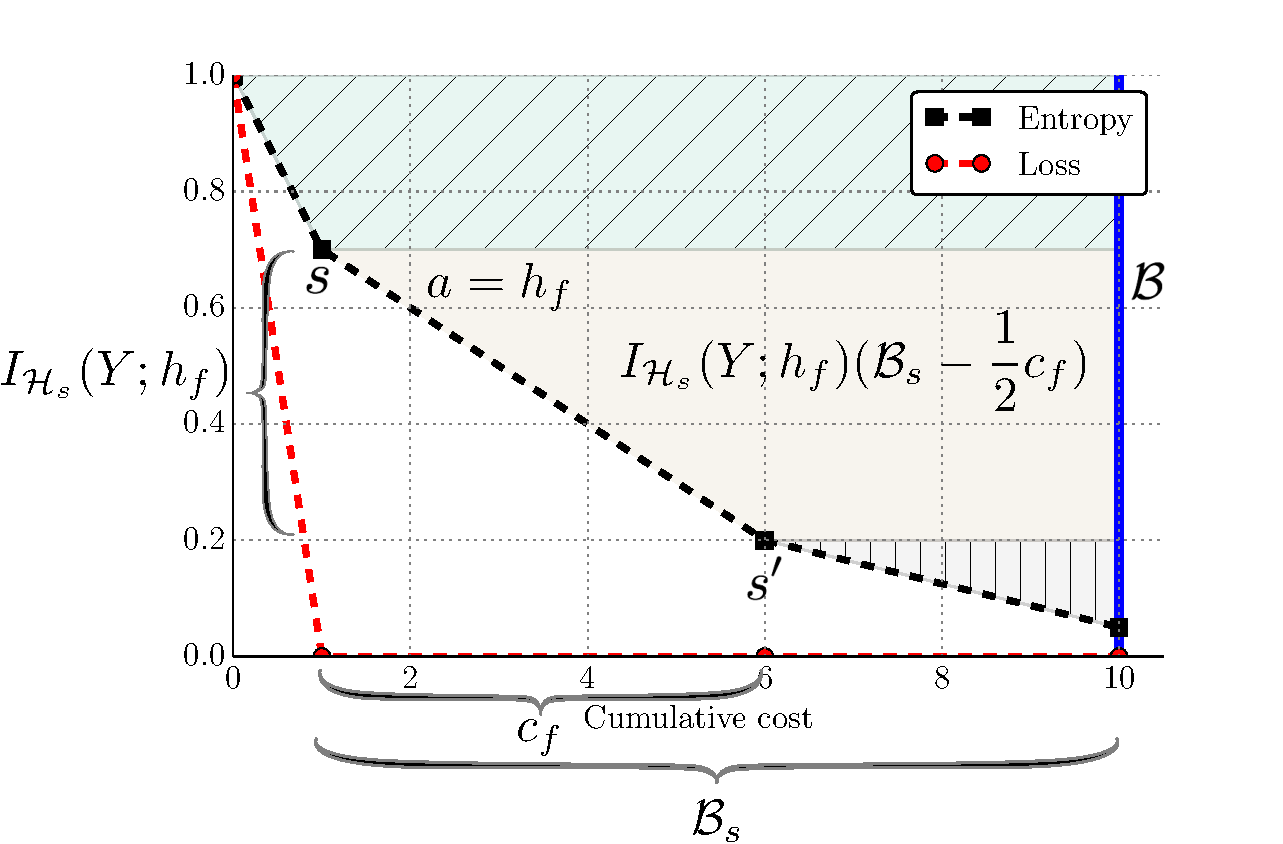
\includegraphics[width=1\linewidth]{../../figures/rewards.pdf}
\caption{
Definition of the reward function.
To maximize the total area above the entropy vs. cost curve from $0$ to $\mathcal{B}$, we define the reward of an individual action as the area of the slice of the total area that it contributes.
From state $s$, action $a = h_f$ leads to state $s'$ with cost $c_f$.
The information gain is $I_{\mathcal{H}_s}(Y; h_f) = H(Y; \mathcal{H}_s) - H(Y; \mathcal{H}_s \cup {h_f})$.
\label{fig:rewards}}
\end{figure}

\begin{mydef} \label{def:problem}
\textbf{The test-time efficient multi-class classification problem} consists of

\begin{itemize}
\addtolength{\itemsep}{-.55\baselineskip}
\item
$N$ instances labeled with one of $K$ labels: ${\mathcal{D} = \{x_n \in \mathcal{X}, y_n \in \mathcal{Y} = \{1, \dots, K\}\}_{n=1}^N}$.

\item
$F$ features $\mathcal{H} = \{h_f : \mathcal{X} \mapsto \mathbb{R}^{d_f} \}_{f=1}^F$, with associated costs $c_f$.

\item Budget-sensitive loss $\mathcal{L}_\mathcal{B}$, composed of cost budget $\mathcal{B}$ and loss function ${\ell(\hat{y}, y) \mapsto \mathbb{R}}$.
\end{itemize}

The goal is to find a \textbf{feature selection} policy $\pi(x): \mathcal{X} \mapsto 2^\mathcal{H}$ and a \textbf{feature combination} classifier $g(\mathcal{H}_\pi) : 2^\mathcal{H} \mapsto \mathcal{Y}$ such that such that the total budget-sensitive loss $\sum \mathcal{L}_\mathcal{B}(g(\pi(x_n)), y_n)$ is minimized.
\end{mydef}

%The features $h_f$ can be classifier outputs, possibly multi-class; following convention, we refer to such features as \emph{weak learners}.

The cost of a selected feature subset $\mathcal{H}_{\pi(x)}$ is $C_{\mathcal{H}_\pi(x)}$.
The budget-sensitive loss $\mathcal{L}_\mathcal{B}$ presents a \textbf{hard budget constraint} by only accepting answers with $C_{\mathcal{H}} \leq \mathcal{B}$.
Additionally, $\mathcal{L}_\mathcal{B}$ can be \textbf{cost-sensitive}: answers given with less cost are more valuable than costlier answers.
The motivation for the latter property is \emph{Anytime} performance; we should be able to stop our algorithm's execution at any time and have the best possible answer.

Feature costs $c_f$ can be specified flexibly, with options including theoretical analysis, number of flops, wall clock runtime, total CPU time, or exact power expenditure.
We believe that a deployment in a modern datacenter is most likely to optimize for power expenditure.
In the absence of reliable ways to measure power, we use total CPU time to define the cost: if an operation is performed in parallel on multiple cores, its cost is considered to be the total cpu time on all cores.

% For a weak learner $h_f$, the cost $c_f$ is composed of the cost of an underlying feature extraction $\phi_{h_f}(x)$ and the cost of subsequent classification.
% Once $h_f$ is computed, its underlying feature $\phi$ is considered to be free for all other features $h_f'$ that share it, if any, such that $c_f' < c_f$.
% Note that in state-of-the-art object recognition systems, complex features and feature encodings are often followed by linear classifiers, and feature extraction cost dominates the total cost.

% \todo{REDO this:}
% A quick preview of an instance of the defined problem is in order.
% On the ImageNet dataset, we could define $h_f$ as intersections of feature channels and class subsets:\\
% {\footnotesize\texttt{
% GIST.Animal, SIFT-BOW.Animal, LLC-SIFT.Animal,\\
% GIST.Vehicle, SIFT-BOW.Vehicle, LLC-SIFT.Vehicle.}}\\
% $\mathcal{G}$ could be defined by a hierarchical loss (accuracy at the leaf nodes counts more than accuracy at inner nodes), and $\mathcal{B}$ could only admit answers that take less than 5 seconds.

At training time, our computation is unbudgeted, and we can compute all features to have \emph{fully-observed} training instances.
At test time, there is a budget and so the instances we classify will only be \emph{partially-observed}, as determined by the feature selection policy.

We defer discussion of learning the \textbf{feature combination} classifier $g(\mathcal{H}_\pi) : 2^\mathcal{H} \mapsto \mathcal{Y}$ to~\autoref{sec:classifier}.
For now, we assume that $g$ can combine an arbitrary subset of features and provide a distribution $P(Y = y)$.
For example, $g$ could be a Naive Bayes (NB) model trained on the fully-observed data.

% \subsection{Static greedy selection.}
% Our initial goal is select a feature subset $\pi(x)$ such that $C_{\pi(x)} \leq \mathcal{B}$ and $\sum \ell(g(\pi(x_n)), y_n)$ is minimized.
% We assume that given a feature subset $\pi(x)$, we are able to find a classifier function $g$ such that the loss is minimized.

% If the classifier $g$ can give a full distribution $P(Y = y)$ and not just a prediction $y \in \{1, \dots, K\}$, we can maximize information gain of the selected subset, instead of directly minimizing the loss of $g(\pi(x))$:\[
% I(Y; \pi(x)) = H(Y) - H(Y | \pi(x)) = \sum_{y \in Y} P(y) \log P(y) -  \sum_{\substack{y \in Y,\\z \in Z}} P(y, z) \log P(y \mid z)
% \]
% To the extent that $g$ is unbiased, maximizing information gain corresponds to minimizing loss, and has the benefit of ensuring that we not only make the right classification decision but also become maximally certain.

% Finding the optimal subset is NP-hard.
% A common heuristic is simple greedy selection, which is known to be near-optimal for optimizing submodular set functions with unit-cost elements \parencite{Nemhauser-1978}.
% In case of non-uniform additive costs, it can be proven that when all features $h$ are independent given $Y$ (as in an NB classifier), building $\pi(x)$ by repeatedly selecting
% \begin{align*}
% h* = \argmax_{h \in \mathcal{H} \setminus \pi(x)} \frac{1}{c_f} \left[ H(h \mid \pi(x)) - H(h \mid Y) \right]
% \end{align*}
% while $C_{\pi(x)} \leq \mathcal{B}$ gives $I(Y; \pi(x)) \geq \frac{1}{2} (1 - 1/e) I_{\text{OPT}}$ with additional terms if the entropy calculation is not exact \parencite{Krause-UAI-2005}\footnote{A tighter (by factor of 2) bound is possible with a $O(F^5)$ instead of this $O(F^2)$ algorithm \parencite{Krause-note-2005}.}.

% However, we may find the feature independence assumption too restrictive or may not be able to reliably compute entropy.
% Additional difficulties come from introducing a setup cost or non-additive costs \todo{although we could resolve them.}
% When we make the feature selection dynamic---guided by the feature values observed---we will face further challenges if the structure of the problem necessitates a non-myopic solution.
% \todo{Need stronger explanation for why we are not proceeding with adaptive submodularity---or just not mention submodularity at all?}

\subsection{Dynamic feature selection as a Markov-Decision-Process (MDP).}
To model the \textbf{feature selection} policy $\pi(x): \mathcal{X} \mapsto 2^\mathcal{H}$, we introduce the Markov Decision Process (MDP), which defines a single \emph{episode} of selecting features for some instance $x$.

\begin{mydef} \label{def:MDP}
The \textbf{feature selection MDP} consists of the tuple $(\mathcal{S}, \mathcal{A}, T(\cdot), R(\cdot), \gamma)$:

\begin{itemize}\addtolength{\itemsep}{-.55\baselineskip}
\item \textbf{State} $s \in \mathcal{S}$ stores the selected feature subset $\mathcal{H}_{\pi(x)}$ and their values and total cost $C_{\mathcal{H}_{\pi(x)}}$.
\item The set of \textbf{actions} $\mathcal{A}$ is exactly the set of features $\mathcal{H}$.
\item The (stochastic) \textbf{state transition} distribution $T(s' \mid s, a)$ can depend on the instance $x$.
\item The \textbf{reward} function $R(s, a, s') \mapsto \mathbb{R}$ is manually specified, and depends on the classifier $g$ and the instance $x$.
\item The discount $\gamma$ determines amount of \textbf{lookahead} in selecting actions: if 0, actions are selected greedily based on their immediate reward; if 1, the reward accrued by subsequent actions is given just as much weight as the reward of the current action.
\end{itemize}
\end{mydef}

Running the MDP on a given instance $x$ gives a trajectory $\xi = (s_0, a_0, s_1, r_1, \dots, a_{I-1}, s_I, r_I)$, where $I$ is the total number of actions taken (and therefore features selected), $s_0$ is the initial state, $a_i \sim \pi(a \mid s_i)$ is chosen by the \emph{policy} $\pi(a \mid s)$, and $s_{i+1} \sim T(s \mid s_i, a_i)$, which can depend on $x$.
The total expected reward (value) of an MDP episode is written as
\begin{equation} \label{eq:expected_reward}
V_\pi(s_0) =
\mathbb{E}_{\xi \sim \left\{ \pi, x \right\}} r(\xi) =
\mathbb{E}_{\xi \sim \left\{ \pi, x \right\}} \left[ \sum_{i=0}^I \gamma^i \, r_i \right]
\end{equation}
Gathering such trajectories forms the basis of our policy learning method.

\subsection{Defining the reward.}
The budget-sensitive loss $\mathcal{L}_\mathcal{B}$ enforces \emph{Anytime} performance by valuing early gains more than later gains.
To formalize this, consider \hyperref[fig:rewards]{Figure~\ref*{fig:rewards}}, which shows the entropy and the 0-1 loss of $g$ at every point in a sequential feature selection episode for some instance $x$.
For the best \emph{Anytime} performance, we want to capture the most area above the loss vs. cost curve, up to max budget $\mathcal{B}$ \parencite{Karayev-NIPS-2012}.

Recall from \eqref{eq:expected_reward} that the value of an episode $\xi$ is defined as the sum of obtained rewards.
If the reward of a single action is defined as the area above the curve that is captured as a direct result, then the value of the whole episode exactly corresponds to $\mathcal{L}_\mathcal{B}$.

However, there is a problem with using loss directly: only the first action to ``tip the scale'' toward the correct prediction gets a direct reward (in the figure, it is the first action).  A smoother reward function is desirable:
if the classifier $g$ can give a full distribution $P(Y = y \mid \mathcal{H}_{\pi(x)})$ and not just a prediction $\hat{y} \in \mathcal{Y}$, we can maximize the \emph{information gain} of the selected subset instead of directly minimizing the loss of $g(\pi(x))$:
\begin{eqnarray}
I(Y; \mathcal{H}_{\pi(x)}) &=& H(Y) - H(Y | \mathcal{H}_{\pi(x)}) = \\ \notag
&=& \sum_{y \in Y} P(y) \log P(y) -  \\ \notag
&&\sum_{y, \mathcal{H}_{\pi(x)}} P(y, \mathcal{H}_{\pi(x)}) \log P(y \mid \mathcal{H}_{\pi(x)})
\end{eqnarray}
To the extent that $g$ is unbiased, maximizing information gain corresponds to minimizing loss, and ensures that we not only make the right classification decision but also become maximally certain.
Therefore, as graphically presented in \hyperref[fig:rewards]{Figure~\ref*{fig:rewards}}, we define the reward of selecting feature $h_s$ with cost $c_f$ with the set $\mathcal{H}_s$ computed to be $I_{\mathcal{H}_s}(Y; h_f) (\mathcal{B}_s - \frac{1}{2}c_f)$.

Although we do not evaluate in this regime, note that this definition easily incorporates a \textbf{setup cost} in addition to \textbf{deadline cost} by only computing the area in between setup and deadline costs.

\subsection{Parametrizing and learning the policy.}
% From the trajectories we can compute the \emph{value function} for any state:
% \begin{equation} \label{eq:value_function}
% V_\pi(s) = \sum_{s'} T_\pi(s, s') \left[ R_\pi(s, s') + \gamma V_\pi(s') \right]
% \end{equation}

Space constraints prohibit a full exposition of reinforcement learning techniques; \parencite{Sutton1998} provides a thorough review.
In brief: we seek $\pi$ that maximizes the expected value of the MDP \eqref{eq:expected_reward}.
Therefore, actions must be selected according to their expected \emph{value}:
\begin{align*}
\argmax_a \pi(a \mid s) = \argmax_a Q^*(s,a)
\end{align*}
where $Q^*(s,a)$ is the optimal \emph{action-value function}---the expected value of taking action $a$ in state $s$ and then acting optimally to the end of the episode.

Because the state represents an exponential number of subsets and associated real values, we cannot represent $Q(s,a)$ exactly.
Instead, we use feature approximation and write $Q(s,a) = \theta^T \phi(s, a)$,  where $\phi: \mathcal{S} \times \mathcal{A} \mapsto \mathbb{R}^{d_s}$ is the state featurization function, $d_s$ is the dimensionality of the state feature vector, and $\theta$ is a vector of weights that defines the policy.

Specifically, the policy is defined as
\begin{equation}
\pi(a \mid s) = \frac{1}{Z} \exp\left(\frac{1}{\tau} \theta^T \phi(s, a)\right)
\end{equation}
where $Z$ is the appropriate normalization and $\tau$ is a temperature parameter that controls the level of exploration vs. exploitation in the policy.
As $\tau \rightarrow 0$, ${\pi(a \mid s)}$ becomes highly peaked at $\argmax_a Q(s,a)$; it becomes uniform as $\tau \rightarrow \infty$.

As commonly done, we learn the $\theta$ by \emph{policy iteration}.
First, we gather $(s, a, r, s')$ samples by running episodes (to completion) with the current policy parameters $\theta_i$.
From these samples, $\hat{Q}(s, a)$ values are computed, and $\theta_{i+1}$ are given by $L_2$-regularized least squares solution to $\hat{Q}(s, a) = \theta^T \phi(s, a)$, on all states that we have seen in training.

During training, we gather samples starting from either a random feasible state, with probability $\epsilon$, or from the initial empty state otherwise.
Both $\epsilon$ and $\tau$ parameters decay exponentially with the number of training iterations.
Training is terminated if $\pi_{\theta_{i+1}}$ returns the exact same sequence of episodes $\xi$ on a validation set as $\pi_{\theta_{i}}$.

\paragraph{Static vs. Dynamic state-action feature vector.}\label{sec:policy_features}
The featurization function $\phi(s)$ extracts the following features from the state:
\begin{itemize}\addtolength{\itemsep}{-.5\baselineskip}
\item Bit vector $\textbf{m}$ of length $F$: initially all bits are $1$ and are set to $0$ when the corresponding feature is computed.
\item For each $h_f$, a vector of size $d_f$ representing the values; $0$ until observed.
\item Cost feature $c \in [0, 1]$, for fraction of the budget spent.
\item Bias feature $1$.
\end{itemize}

\begin{algorithm}[]
\SetKwFunction{ComputeRewards}{ComputeRewards}
\SetKwFunction{GatherSamples}{GatherSamples}
\SetKwFunction{UpdatePolicy}{UpdatePolicy}
\SetKwFunction{UpdateClassifier}{UpdateClassifier}

\SetAlgoLined
\KwIn{$\mathcal{D} = \{x_n, y_n\}_{n=1}^N$; $\mathcal{L}_\mathcal{B}$}
\KwResult{Trained $\pi$, $g$}
\BlankLine
$\pi_0 \leftarrow$ random\;
\For {$i \leftarrow 1$ \KwTo max\_iterations} {
    States, Actions, Costs, Labels $\leftarrow$ \GatherSamples{$\mathcal{D}$, $\pi_{i-1}$}\;
    $g_i \leftarrow$ \UpdateClassifier{States, Labels}\;
    Rewards $\leftarrow$ \ComputeRewards{States, Costs, Labels, $g_i, \mathcal{L}_\mathcal{B}, \gamma$}\;
    $\pi_i \leftarrow$ \UpdatePolicy{States, Actions, Rewards}\;
}
\caption{Because reward computation depends on the classifier, and the distribution of states depends on the policy, $g$ and $\pi$ are trained iteratively.\label{alg:learning}}
\end{algorithm}

These features define the \textbf{dynamic} state, presenting enough information to have a \emph{closed-loop} (dynamic) policy that may select different features for different test instances.
The \textbf{static} state has all of the above features except for the observed feature values.
This enables only an \emph{open-loop} (static) policy, which is exactly the same for all instances.
Policy learned with the static state is used as a baseline in experiments.

The state-action feature function $\phi(s, a)$ effectively block-codes these features: it is $0$ everywhere except the block corresponding to the action considered.
In implementation, we train $F$ separate regressions with a tied regularization parameter, which is K-fold cross-validated.

\paragraph{Effect of $\gamma$.}
Note that solving the MDP with these features and with $\gamma=0$ finds a \textbf{Static, greedy} policy: the value of taking an action in a state is exactly the expected reward to be obtained.
When $\gamma=1$, the value of taking an action is the entire area above the curve as defined in \autoref{fig:rewards}, and we learn the \textbf{Static, non-myopic} policy---another baseline.

\subsection{Learning the classifier.}\label{sec:classifier}

We have so far assumed that $g$ can combine an arbitrary subset of features and provide a distribution $P(Y = y)$---for example, a Gaussian Naive Bayes (NB) model trained on the fully-observed data.
% However, a Naive Bayes classifier suffers from its restrictive independence assumptions.

Since discriminative classifiers commonly provide better performance, we use a \textbf{logistic regression} classifier, which presents a new challenge:
% bu have to account for missing data:
at test time, some feature values are missing and need to be imputed.
If the classifier is trained exclusively on fully-observed data, then the feature value statistics at test time will not match, resulting in poor performance.
Therefore, we need to learn classifier weights on a distribution of data that exhibits the pattern of missing features induces by the policy $\pi$.
At the same time, learning the policy depends on the classifier $g$, used in the computation of the rewards.
For this reason, the policy and classifier need to be learned jointly: \autoref{alg:learning} gives the iterative procedure.

\paragraph{Unobserved value imputation.}
Unlike the Naive Bayes classifier, the logistic regression classifier is not able to use an arbitrary subset of features $\mathcal{H}_\pi$, but instead operates on feature vectors of a fixed size.
To represent the feature vector of a fully observed instance, we write $\mathbf{x} = [h_1(x), \dots, h_f(x)]$.
In case that $\mathcal{H}_\pi \subset \mathcal{H}$, we need to fill in unobserved feature values in the vector.

A basic strategy is \textbf{mean imputation}: filling in with the mean value of the feature:
\begin{align}
\mathbf{x}_\pi = \left[ h_i(x) : \left\{ \begin{array}{rl}
 h_i(x) &\mbox{ if $h_i \in \mathcal{H}_{\pi(x)}$} \\
 \bar{\mathbf{h}}_i &\mbox{ otherwise}
\end{array} \right. \right]
\end{align}

If we assume that $\mathbf{x}$ is distributed according to a multivariate Gaussian $\mathbf{x} \sim \mathcal{N}(\mathbf{0}, \Sigma)$, where $\Sigma$ is the sample covariance $X^T X$ and the data is standardized to have zero mean, then it is possible to do \textbf{Gaussian imputation}.
Given a feature subset $\mathcal{H}_\pi$, we write:
\begin{equation}
\mathbf{x}_\pi = \begin{bmatrix} \mathbf{x}^\text{o}\\  \mathbf{x}^\text{u} \end{bmatrix} \sim \mathcal{N} \left( \mathbf{0}, \begin{bmatrix} \mathbf{A} & \mathbf{C}\\ \mathbf{C}^T & \mathbf{B} \end{bmatrix} \right)
\end{equation}
where $\mathbf{x}^\text{o}$ and $\mathbf{x}^\text{u}$ represent the respectively observed and unobserved parts of the full feature vector $\mathbf{x}$.
%, $\mathbf{A}$ is the covariance matrix of $\mathbf{x}^\text{o}$, $\mathbf{B}$ is the covariance matrix of $\mathbf{x}^\text{u}$, and $C$ is the cross-variance matrix that has as many rows as the size of $\mathbf{x}^\text{o}$ and as many columns as the size of $\mathbf{x}^\text{u}$.
%\parencite{Roweis-gaussian-identities}.
In this case, the distribution over unobserved variables conditioned on the observed variables is given as
$\mathbf{x}^\text{u} \mid \mathbf{x}^\text{o} \sim \mathcal{N} \left( \mathbf{C}^T \mathbf{A}^{-1} \mathbf{x}^\text{o},\, \mathbf{B} - \mathbf{C}^T \mathbf{A}^{-1} \mathbf{C} \right)$.

\paragraph{Learning more than one classifier.}
As illustrated in \hyperref[fig:state_space]{Figure~\ref*{fig:state_space}}, the policy $\pi$ selects some feature subsets more frequently than others.
Instead of learning only one classifier $g$ that must be robust to all observed feature subsets, we can learn several classifiers, one for each of the most frequent subsets.
This is done by maintaining a distribution over encountered feature subsets during training.
For each of the $K$ most frequent subsets, a separate classifier is trained, using data that is closest by Hamming distance on the selected-feature bit vector.

Each classifier is trained with the \textsc{Liblinear} implementation of logistic regression, with $L_2$ regularization parameter K-fold cross-validated at each iteration.

\begin{figure}[ht]
\centering
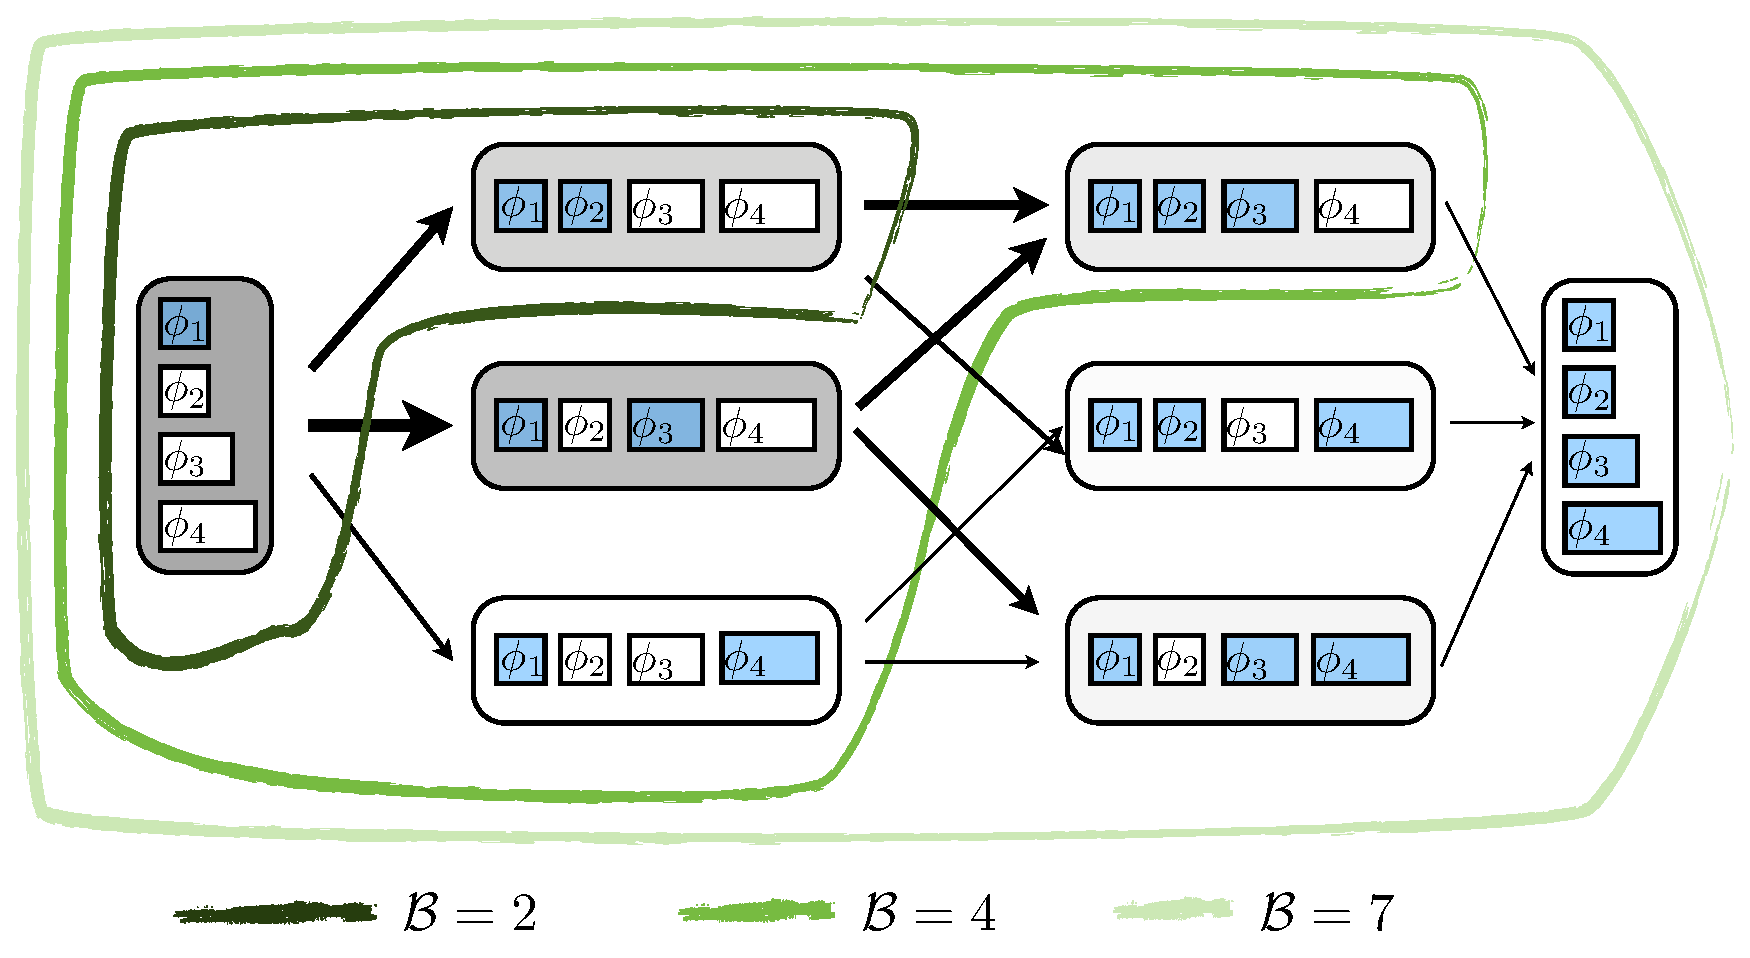
\includegraphics[width=1\linewidth]{../../figures/mdp_masks.pdf}
\caption{
The action space $\mathcal{A}$ of the MDP is the the set of features $\mathcal{H}$, represented by the $\phi$ boxes.
The primary discretization of the state space can be visualized by the possible feature subsets (larger boxes); selected features are colored in the diagram.
The feature selection policy $\pi$ induces a distribution over feature subsets, for a dataset, which is represented by the shading of the larger boxes.
Not all states are reachable for a given budget $\mathcal{B}$.
In the figure, we show three ``budget cuts'' of the state space.
\label{fig:state_space}
}
\end{figure}

\section{Evaluation}
We evaluate the following sequential selection baselines:
\begin{itemize}\addtolength{\itemsep}{-.35\baselineskip}
\item \textbf{Static, greedy}: corresponds to best performance of a policy that does not observe feature values and selects actions greedily ($\gamma=0$).
\item \textbf{Static, non-myopic}: policy that does not observe feature values but uses the MDP machinery with $\gamma=1$ to consider future action rewards.
\item \textbf{Dynamic, greedy}: policy that observed feature values, but selects actions greedily.
% \item \todo{
% \textbf{Active Classification} \parencite{Gao-NIPS-2011}:
% Feature selection is done by greedy selection based on expected information gain divided by cost (so reward is information gain, $\gamma=0$).
% The feature responses are modeled as a mixture of multivariate Gaussians (one mixture element per class label), and inference is instance-specific, akin to locally weighted regression.
% Feature combination is done by the same model: the posteriors are used as the final answers.
% }
% \item
% \todo{\textbf{MD-DAG} \parencite{Benbouzid-ICML-2012}
% Feature selection is done by an MDP policy with three actions: Skip, Evaluate, Quit over a pre-determined sequence of weak learners (unspecified exactly how the sequence is arranged, except ``by quality'').
% }
\end{itemize}
Our method is the \textbf{Dynamic, non-myopic} policy: observed feature values, and full lookahead.

% In addition to the settings above, we evaluate three additional baselines that do not do any selection at all: (a) \textbf{all} features computed; (b) only the \textbf{best} feature (in terms of $\mathcal{G}$) computed; (c) only the \textbf{least costly} feature computed.

In preliminary experiments, Logistic Regression always performed better than the Gaussian Naive Bayes classifier, and so only the former is used in the experiments below.
As described above, we evaluated classification with \textbf{Gaussian} vs. \textbf{Mean} imputation, and with different number of classifiers (1, 3, and 6) clustered by feature subsets.
We found that mean imputation performed better than Gaussian imputation, and although increased number of classifiers sometimes increased performance, it also made our method more prone to overfitting; $K=1$ classifiers worked best on all tasks.
%For reason of space, we report only the best achieved performance in the following evaluation results.

We evaluate two forms of test-time efficient performance measure: the area under the curve and the performance at max budget, although note that all methods are trained only for the former measure.

While the individual implementation details have been largely provided in the preceding text, here we additionally note that some of our policy and classifier implementations use the scikit-learn package \parencite{Pedregosa2011}.

% \subsection{Baselines}
% \paragraph{Active Classification \parencite{Gao-NIPS-2011}}
% Feature selection is done by greedy selection based on expected information gain divided by cost (so reward is information gain, $\gamma=0$).
% The feature responses are modeled as a mixture of multivariate Gaussians (one mixture element per class label), and inference is instance-specific, akin to locally weighted regression.
% Feature combination is done by the same model: the posteriors are used as the final answers.

% \paragraph{Greedy Miser \parencite{Xu-ICML-2012}}
% Feature selection is done by the CART algorithm \parencite{Breiman-1984} with an impurity function that considers feature cost.
% Feature combination is an ensemble of trees.

% \paragraph{MD-DAG \parencite{Benbouzid-2012-ICML}}
% Feature selection is done by an MDP policy with three actions: Skip, Evaluate, Quit over a pre-determined sequence of weak learners (unspecified exactly how the sequence is arranged, except ``by quality'').
% Feature combination is an unweighted sum.

% \paragraph{Timely \parencite{Karayev-NIPS-2012}}
% Feature selection is done by MDP trained using a state feature vector that has the inference output of an MRF combining feature values.
% Feature combination is done by the same MRF.

\begin{figure*}[ht]
\centering
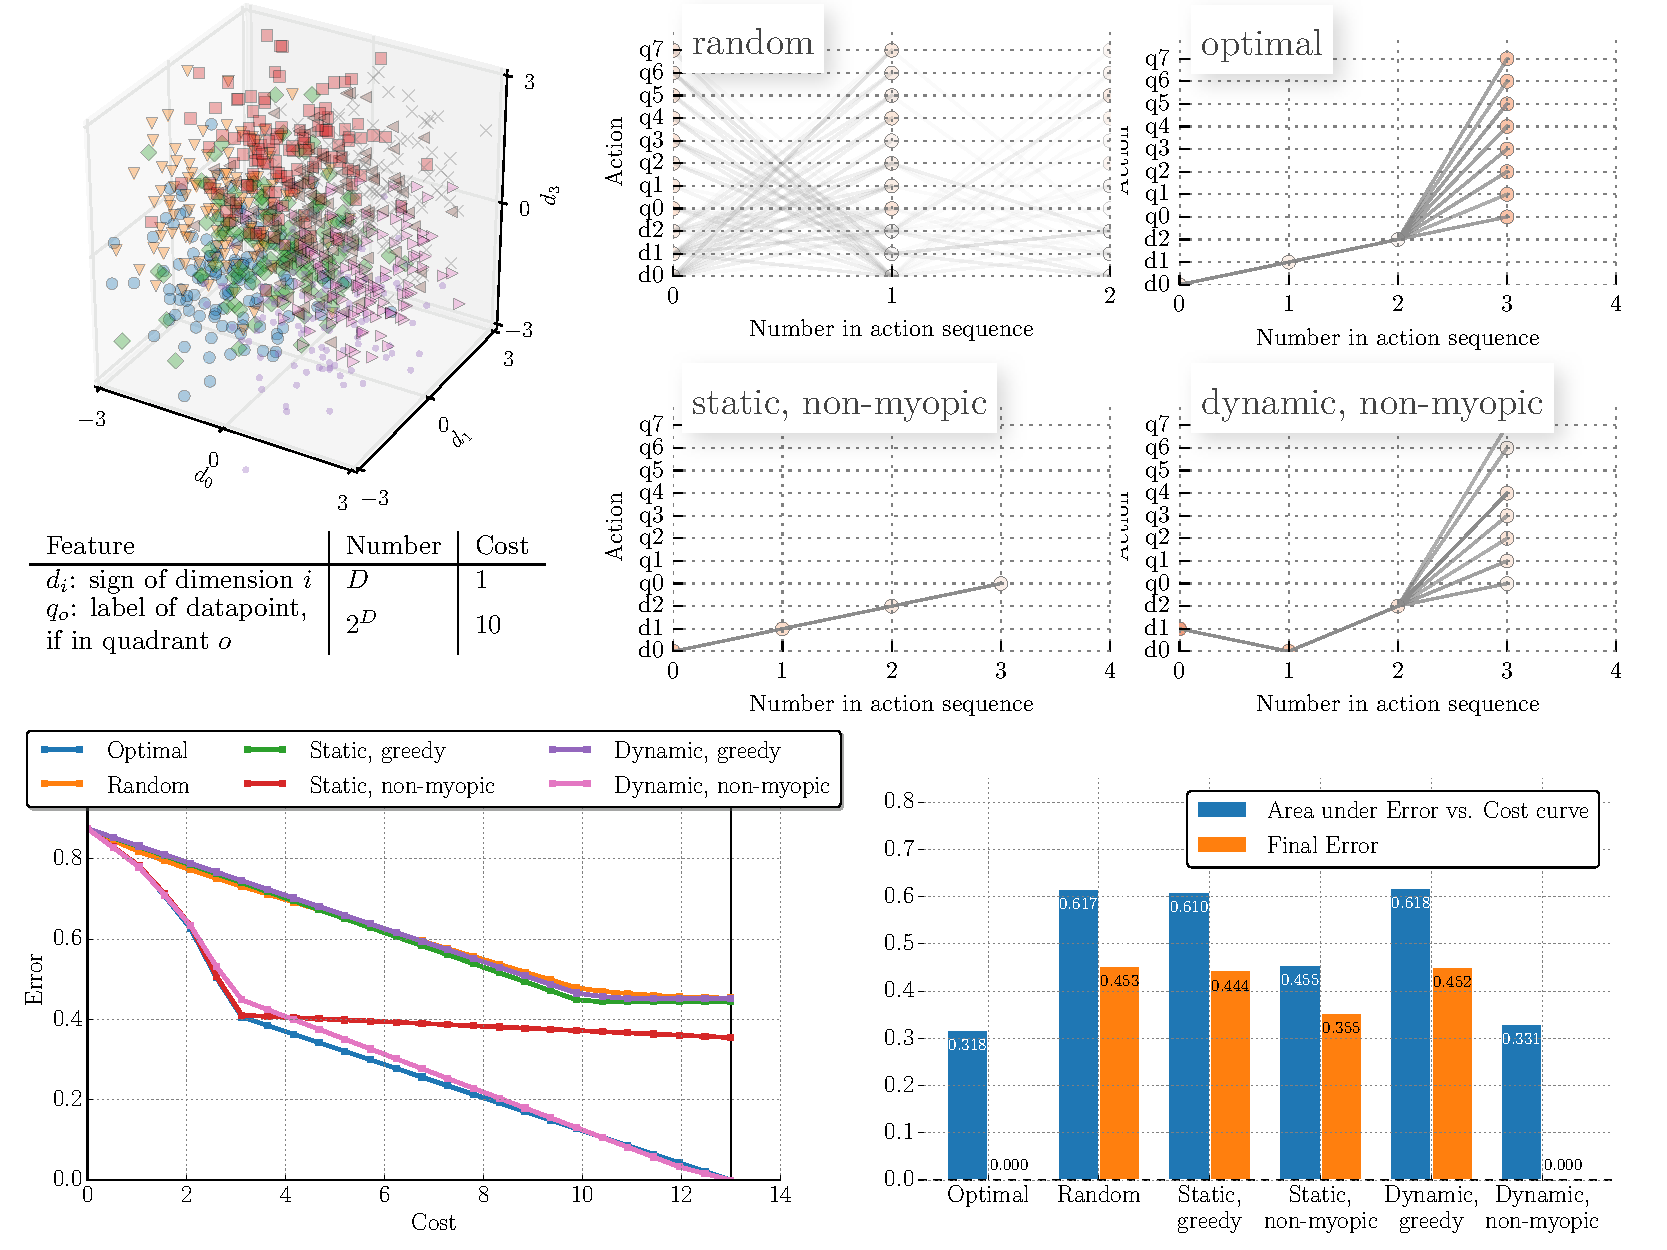
\includegraphics[width=.9\textwidth]{../../figures/synthetic.pdf}
\caption{
Evaluation on the synthetic example (best viewed in color).
The data and the feature costs are shown at top left; the sample feature trajectories of different policies at top right.
(The opacity of the edges corresponds to their prevalence during policy execution; the opacity of the nodes corresponds to the amount of reward obtained in that state.)
Note that the \emph{static, non-myopic} policy correctly learns to select the cheap features first, but is not able to correctly branch, while our \emph{dynamic, non-myopic} approach finds the optimal strategy.
The plots in the bottom half give the error vs. cost numbers.
}

\label{fig:synthetic}
\end{figure*}

\subsection{Synthetic Experiment.}
Following \parencite{Xu-ICML-2013}, we first show that the policy works as advertised in a challenging synthetic example.
In $D$-dimensional space, the data has a label for each of the $2^D$ orthants, and is generated by a unit-variance Gaussian in that orthant (See top left of \autoref{fig:synthetic} for the 3D case).
There are $D$ cheap features that simply return the sign of the data point's coordinate for the corresponding dimension.
For each orthant, there is also an expensive feature that returns the data point's label if the point is located in the corresponding orthant, and random noise otherwise.

The optimal policy on a new data point is to determine its orthant with cheap features, and then take the corresponding expensive action.
Note that both dynamic features and non-myopic learning are crucial to the optimal policy, which is successfully found by our approach.
\autoref{fig:synthetic} shows the results of this optimal policy, a random policy, and of different baselines and our method, trained given the correct minimal budget.

\subsection{Scene recognition.}
The Scene-15 dataset \parencite{Lazebnik-CVPR-2006} contains 4485 images from 15 visual scene classes.
The task is to classify images according to scene.
Following \parencite{Xiao-CVPR-2010}, we extracted 14 different visual features (GIST, HOG, TinyImages, LBP, SIFT, Line Histograms, Self-Similarity, Textons, Color Histograms, and variations).
The features vary in cost from 0.3 seconds to 8 seconds, and in single-feature accuracy from 0.32 (TinyImages) to .82 (HOG).
Separate multi-class linear SVMs were trained on each feature channel, using a random 100 positive example images per class for training.
We used the \texttt{liblinear} implementation, and K-fold cross-validated the penalty parameter $C$.
The trained SVMs were evaluated on the images not used for training, resulting in a dataset of 2238 vectors of 210 confidence values: 15 classes for each of the 14 feature channels.
This dataset was split 60-40 into training and test sets for our experiments.

\hyperref[fig:scenes]{Figure~\ref*{fig:scenes}} shows the results, including learned policy trajectories.
For all evaluated budgets, our \emph{dynamic, non-myopic} method outperforms all others on the area under the error vs. cost curve metric.
Our results on this dataset match the reported results of Active Classification \parencite{Gao-NIPS-2011} (Figure 2) and Greedy Miser \parencite{Xu-ICML-2012} (Figure 3), although both methods use an additional powerful feature channel (ObjectBank)\footnote{Detailed results for this and other experiments are on the project page (see front page for the \href{http://sergeykarayev.com/recognition-on-a-budget/}{link}).}.


\subsection{ImageNet and maximizing specificity.}
The full ImageNet dataset has over 10K categories and over a million images \parencite{Deng-ECCV-2010}.
The classes are organized in a hierarchical structure, which can be exploited for novel recognition tasks.
We evaluate on a 65-class subset introduced in ``Hedging Your Bets'' \parencite{Deng-CVPR-2012}.
In this evaluation, we consider the situation where the initial feature computation has already happened, and the task is to find a path through existing one-vs-all classifiers: features correspond to Platt-scaled SVM confidences of leaf-node classifiers (trained on SIFT-LLC features), and each has cost 1 \parencite{Deng-ECCV-2010}.
Following \parencite{Deng-CVPR-2012}, accuracy is defined on all nodes, and inner node confidences are obtained by summing the probabilities of the descendant nodes.

We combine our sequential feature selection with the ``Hedging Your Bets'' method for backing off prediction nodes using the ImageNet hierarchy to maintain guaranteed accuracy while giving maximally specific answers, given a cost budget.
The results are given in \hyperref[fig:imagenet]{Figure~\ref*{fig:imagenet}}.
As the available budget increases, the \emph{specificity} (defined by normalized information gain in the hierarchy) of our predictions also increases, while accuracy remains constant.
Visualizing this on the ILSVRC-65 hierarchy, we see that the fraction of predictions at the leaf nodes grows with available computation time.
This formulation presents a novel angle on modeling the time course of human visual perception.

\begin{figure*}[ht]
\centering
    \centering
    \begin{subfigure}[b]{0.39\textwidth}
            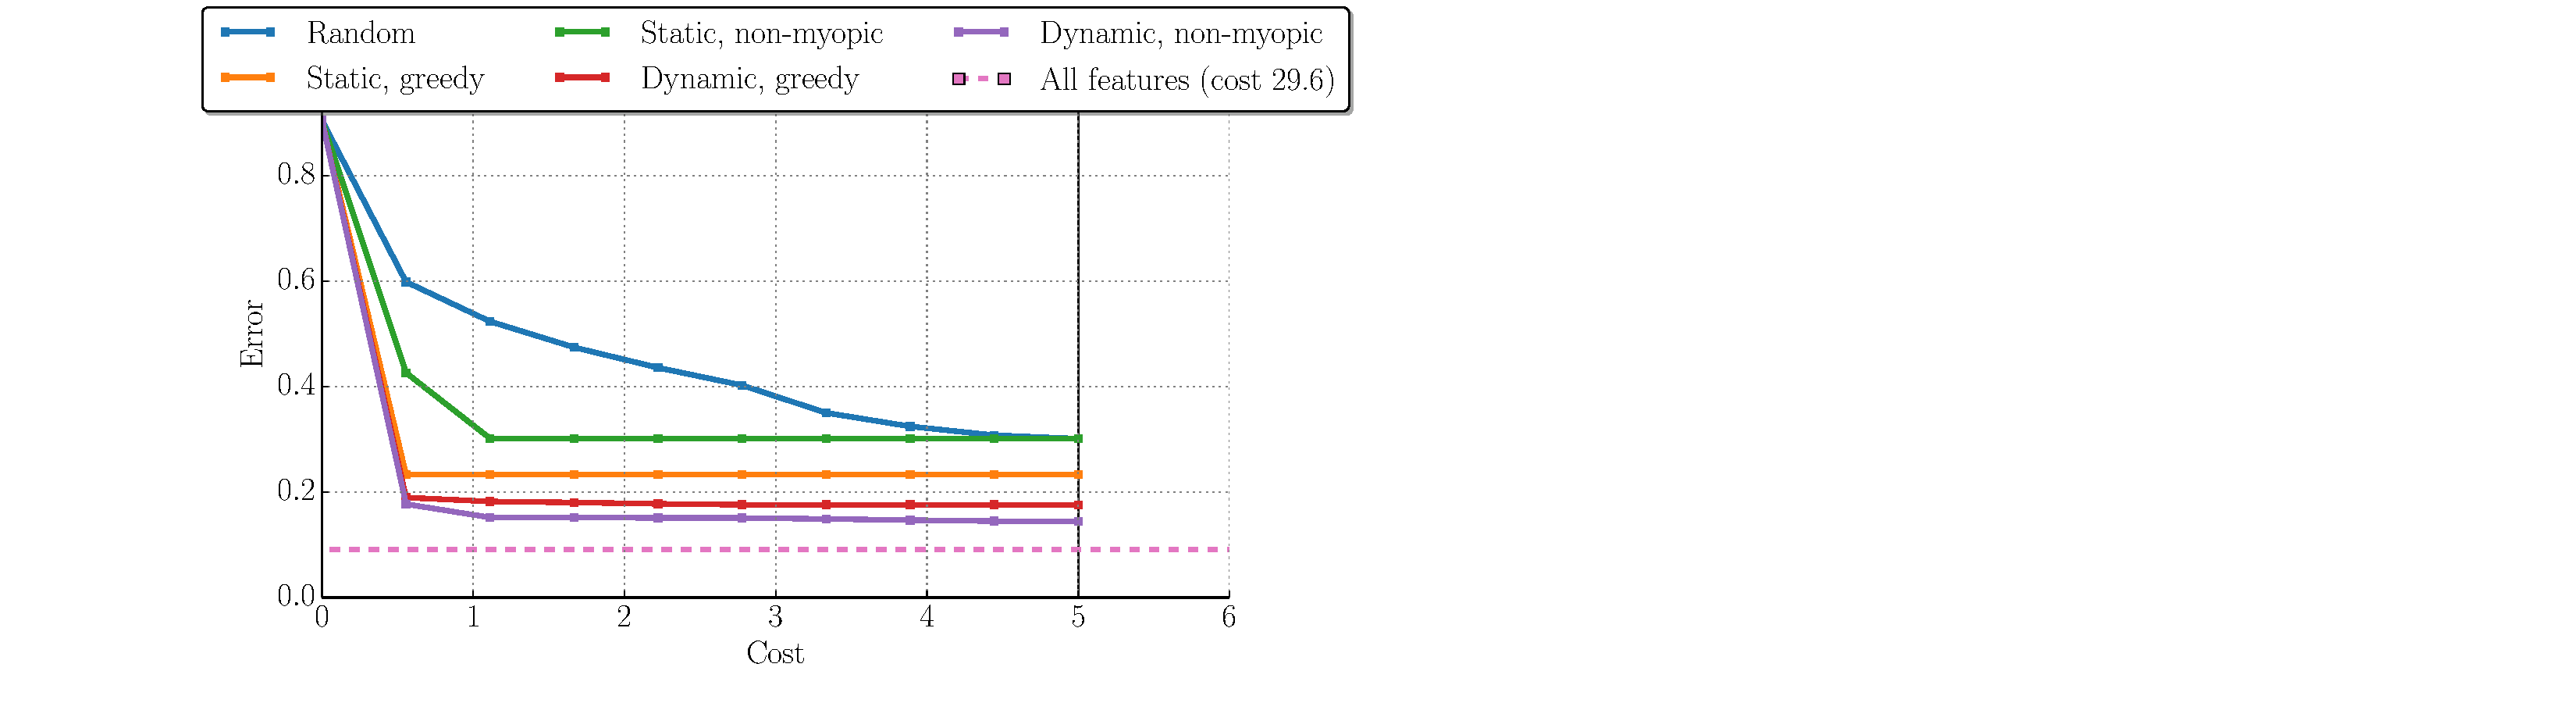
\includegraphics[width=\textwidth]{../../figures/apr11_assembly/scene_15_5_crop.pdf}
            \caption{Error given by policies learned for a budget = 5.}
    \end{subfigure}%
    \begin{subfigure}[b]{0.36\textwidth}
            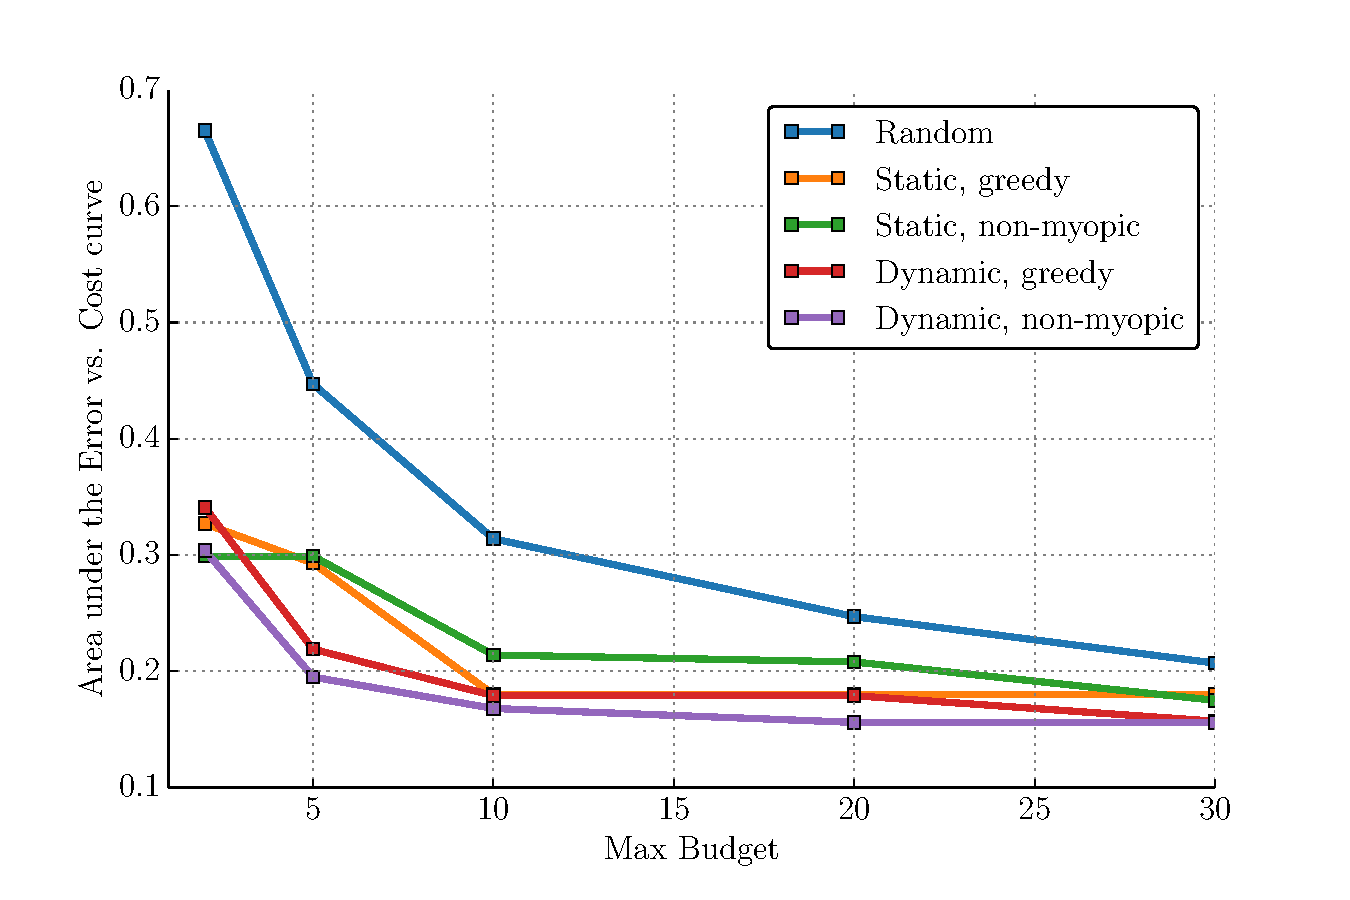
\includegraphics[width=\textwidth]{../../figures/apr11_assembly/_scenes15_auc.pdf}
            \caption{Areas under error vs. cost curves of policies learned at different budgets.}
    \end{subfigure}%
    \begin{subfigure}[b]{0.25\textwidth}
            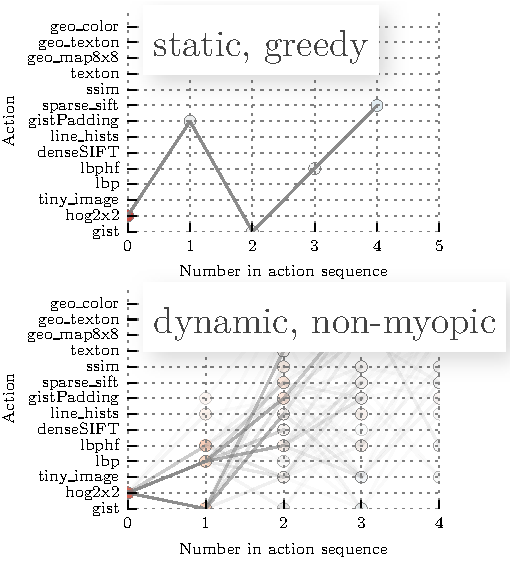
\includegraphics[width=\textwidth]{../../figures/apr11_assembly/scenes_result.pdf}
            \caption{Policy trajectories.}
    \end{subfigure}

    \caption{
Results on Scenes-15 dataset (best viewed in color).
Figure (a) shows the error vs. cost plot for policies learned given a budget of 5 seconds.
Figure (b) aggregates the area under the error vs. cost plot metrics for different policies and budgets, showeing that our approach outperforms baselines no matter what budget it's trained for.
Figure (c) shows the branching behavior of our dynamic policy.
\label{fig:scenes}
    }
\end{figure*}
\begin{figure*}[ht]
\centering
    \begin{subfigure}[b]{0.52\textwidth}
            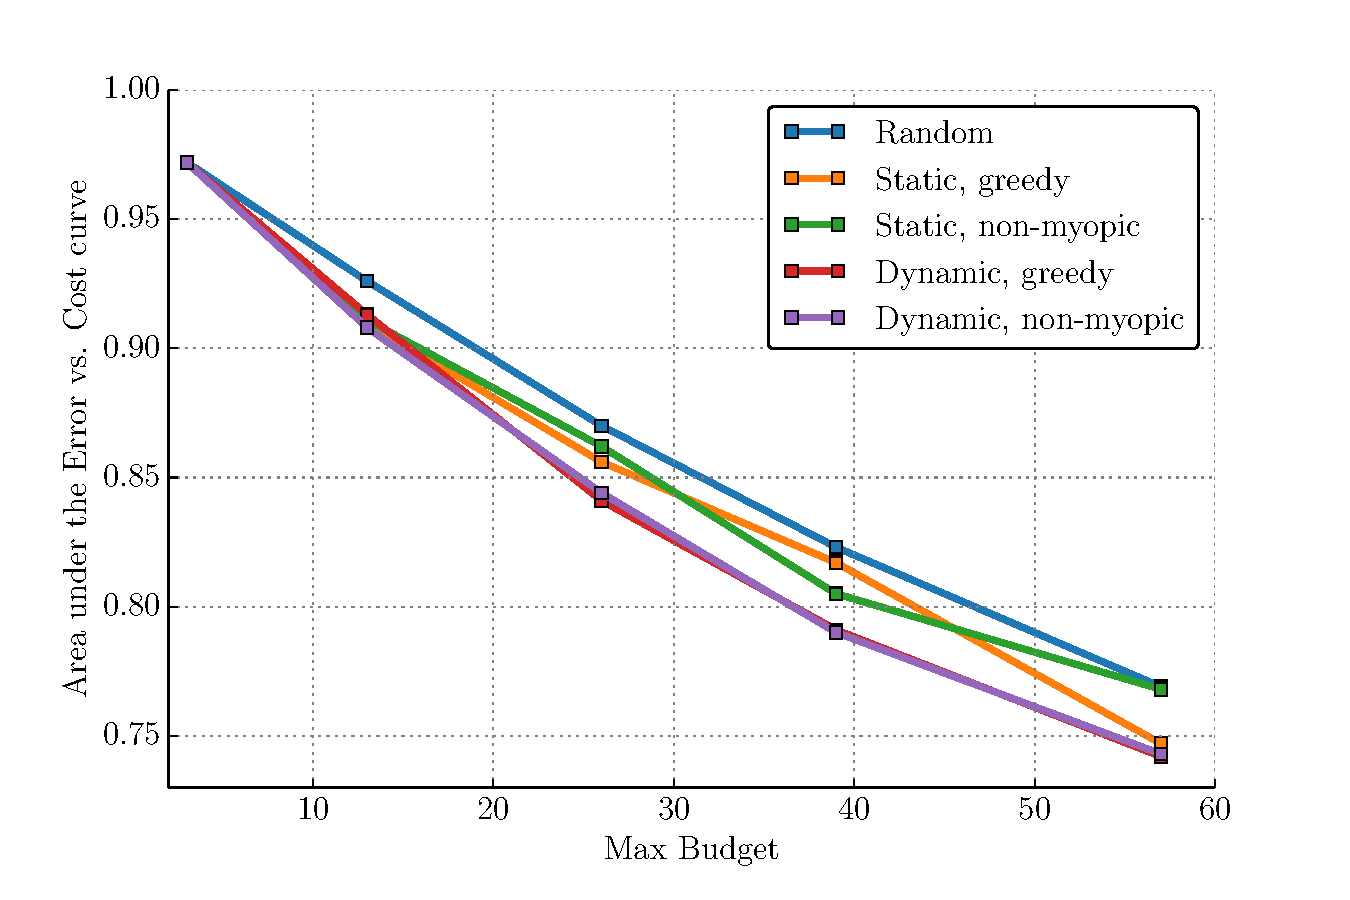
\includegraphics[width=\textwidth]{../../figures/apr11_assembly/_ilsvrc65_auc.pdf}
            \caption{
            Areas under error vs. cost curves for policies learned at different budgets.
            (No specificity back-off is performed here).
            \label{fig:imagenet-a}
            }
    \end{subfigure}\hfill%
    \begin{subfigure}[b]{0.43\textwidth}
            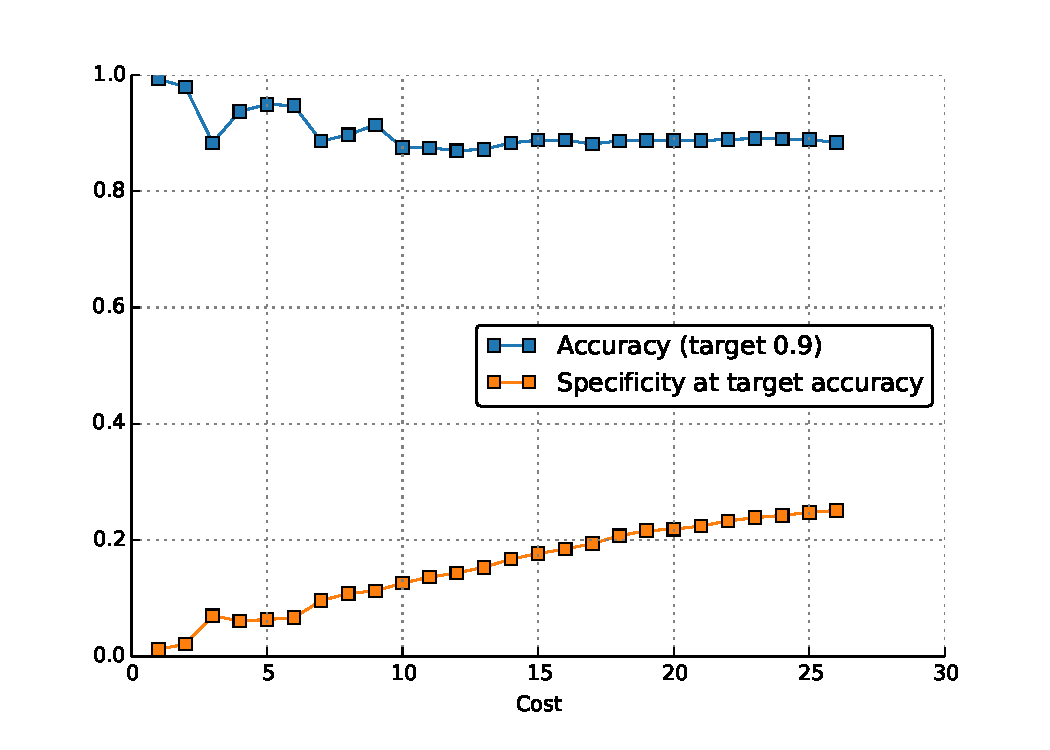
\includegraphics[width=\textwidth]{../../figures/apr11_assembly/ilsvrc65_acc.pdf}
            \caption{
            Holding prediction accuracy constant, we achieve increased specificity with increased cost (on \emph{Dynamic, non-myopic} policy, budget = 36).
            \label{fig:imagenet-b}
            }
    \end{subfigure}\\\vspace{1em}
    \begin{subfigure}[b]{.97\textwidth}
            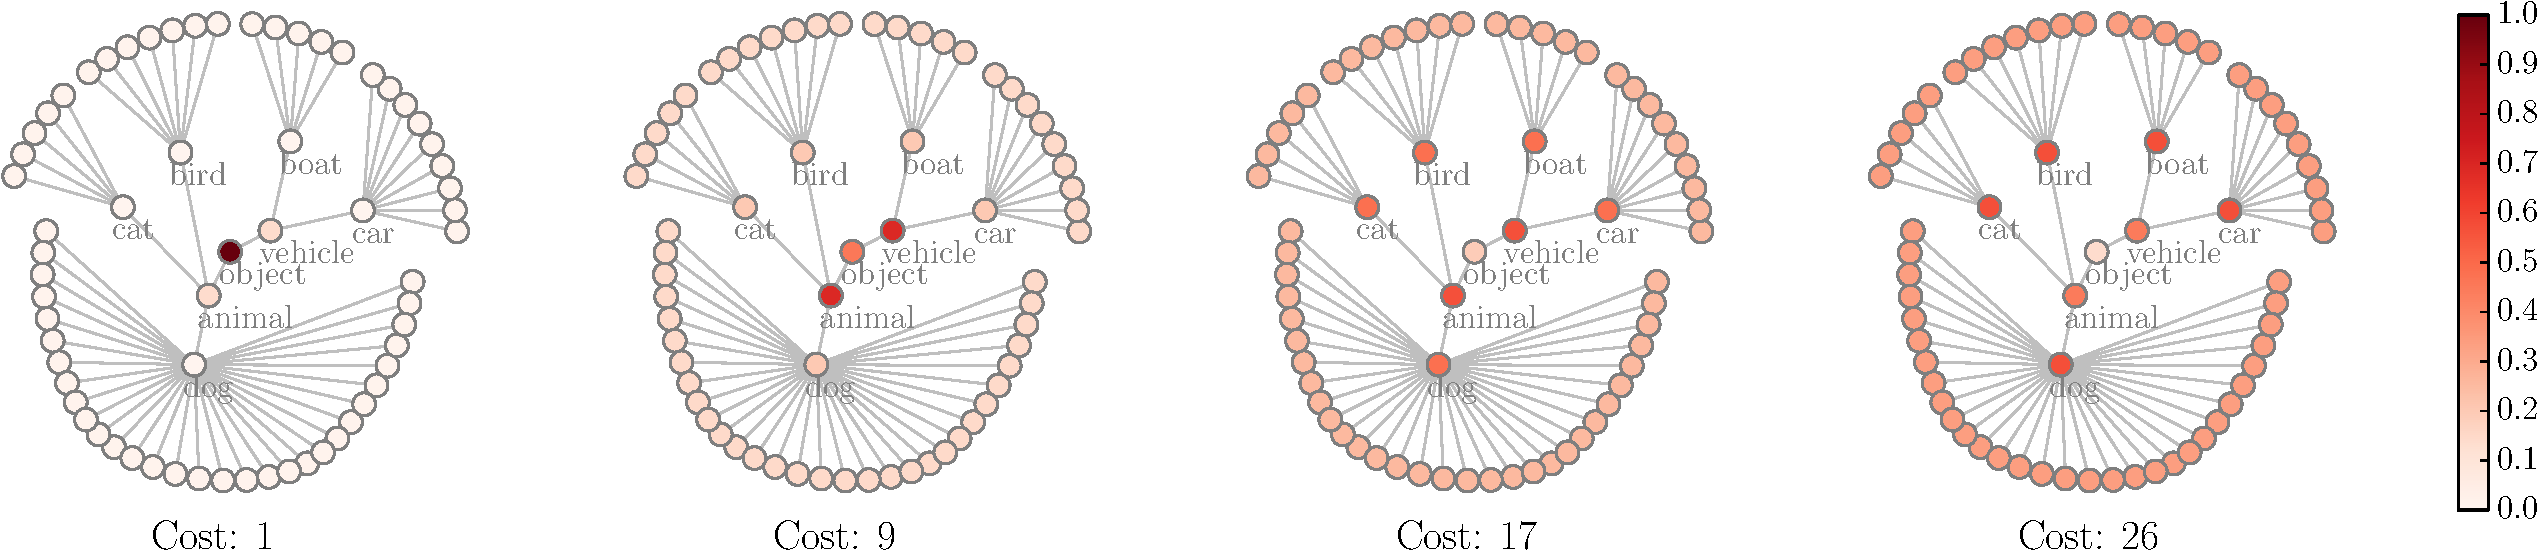
\includegraphics[width=\textwidth]{../../figures/apr11_assembly/ilsvrc65_network-crop.pdf}
            \caption{
            We visualize the fraction of predictions made at inner vs. leaf nodes of ILSVRC-65 at different cost points of an Anytime policy: with more computation, accurate predictions are increasingly made at the leaf nodes.
            \label{fig:imagenet-c}
            }
    \end{subfigure}

\caption{
Results on the ILSVRC-65 dataset (best viewed in color).
Figure (a) shows our dynamic approaches outperforming static baselines for all practical cost budgets.
When our method is combined with Hedging Your Bets \parencite{Deng-CVPR-2012}, a constant prediction accuracy can be achieved at all points in the Anytime policy, with \emph{specificity} of predictions increasing with the cost of predictions.
Figures (b) and (c) show this for the \emph{dynamic, non-myopic} policy learned for budget = 26.
This is analogous to human visual performance, which shows increased specificity at longer stimulus times.
\label{fig:imagenet}}
\end{figure*}

\section{Conclusions and Future Work}
We have shown how to optimize feature selection and classification strategies under an Anytime objective by modeling the associated process as a Markov Decision Process.
Throughout the experiments we show how strategies that adapt the course of computation at test time lead to gains in performance and efficiency.
Beyond the aspects of practical deployment of vision systems that our work is motivated by, we are curious to further investigate our model as a tool to study human cognition and the time course of visual perception.

Lastly, the recent successes of convolutional neural nets for visual recognition open an exciting new avenue for exploring cost-sensitivity.
Layers of a deep network can be seen as features in our system, through which a properly learned policy can optimally direct computation.
